\section{Server}
\subsection{Model}
\begin{figure}[h]
	\centering
	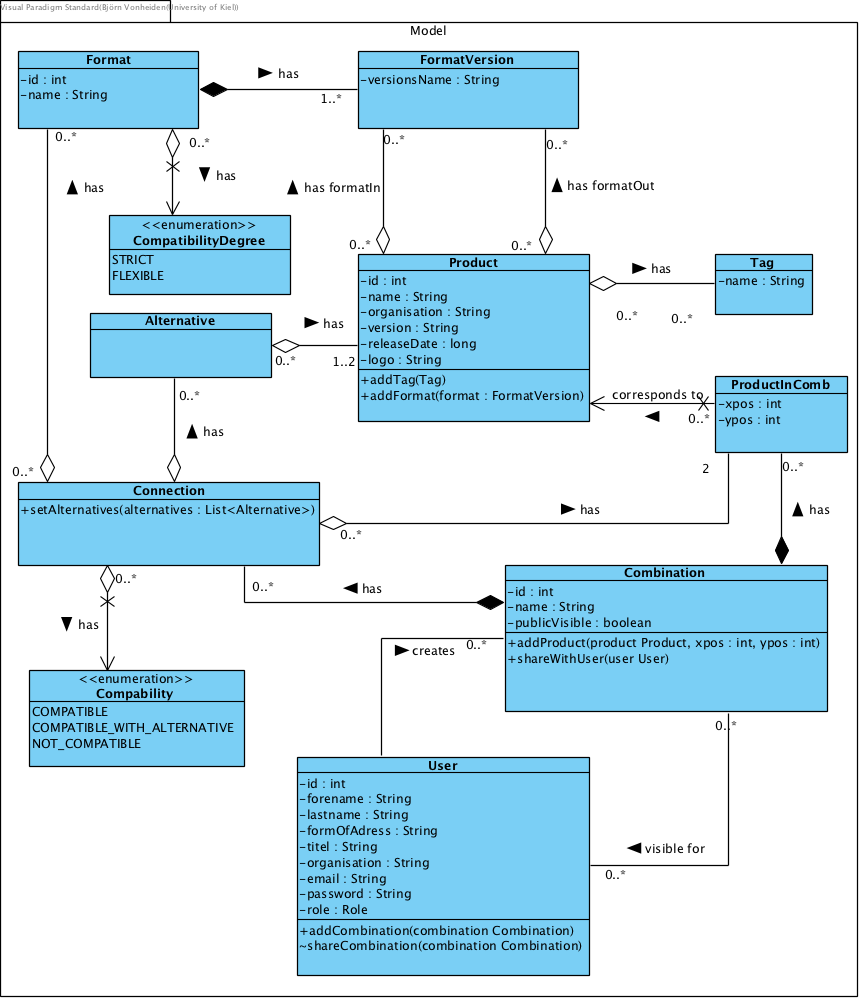
\includegraphics[width=\textwidth]{klassendiagramm/Model}
	\caption{Klassendiagramm - Server - Model}
	\label{fig:klassendiagramm-server-model}
\end{figure}
\begin{table}[h]
	\centering

	\begin{tabularx}{\textwidth}{X X}
		\rowcolor[HTML]{C0C0C0}
		\textbf{Klassenname} & \textbf{Aufgabe} \\
		Model.Alternative & Eine Alternative zu einer Verbindung besteht entweder aus einem oder aus zwei Produkten, welche die Verbindung gültig machen. \\
    	\rowcolor[HTML]{E7E7E7}
    	Model.Combination & Informationen von einer Kombination und Personen, für die die Kombination freigegeben wurde. \\
		Model.Compability  &  Ein Enum, welcher darstellt, ob eine Verbindung kompatibel ist, nicht kompatibel ist oder über eine alternative Kompatibel ist. \\
    	\rowcolor[HTML]{E7E7E7}
		Model.CompatibilityDegree & Ein Enum, welcher entweder 'STRICT' oder 'FLEXIBLE' ist.
		Flexibel heißt, dass das Format abwärts kompatibel ist, strict heißt, dass nur das genau gleiche Format kompatibel ist.\\
		Model.Connection  & Informationen von einer Verbindung. Eine Verbindung hat zwei zugehörige Produkte und eine Richtung.
		Die Richtung wird durch die Reihenfolge der beiden Produkte definiert. \\
    	\rowcolor[HTML]{E7E7E7}
		Model.Format & Ein Format hat eine oder mehrere Versionen und kann entweder strict oder flexible sein. \\
		Model.FormatVersion  & Informationen einer Format-Version.
		Jede Version ist einem Format zugeordnet und hat eine Liste der zugehörigen Produkte, da dies die Suche nach Alternativen effizienter macht.\\
    	\rowcolor[HTML]{E7E7E7}
    	Model.Product & Informationen von einem Dienst.
    	Das Logo wird dabei durch einen Dateipfad definiert. \\
		Model.ProductInComb & Speichert den Ort eines Produktes in einer bestimmten Kombination.
		In einer Kombination kann der selbe Dienst mehrmals vorkommen, dies sind dann aber unterschiedliche ProductInCombs. \\
    	\rowcolor[HTML]{E7E7E7}
		Model.Tag & Ein Tag kann Produkten zugeordnet werden.
		Mithilfe dieser Tags kann nach Produkten gesucht werden. \\
		Model.User & Speichert die Daten eines Benutzers, dessen Combinationen und seine Rolle \\
	\end{tabularx}
	\caption{Klassenbeschreibung - Model}
	\label{table:klassenbeschreibung-model}
\end{table}

\FloatBarrier
\subsection{Logik}
\begin{figure}[h]
	\centering
	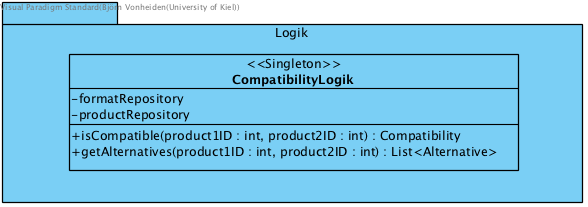
\includegraphics[width=\textwidth]{klassendiagramm/Logik}
	\caption{Klassendiagramm - Logik}
	\label{fig:klassendiagramm-logik}
\end{figure}
\begin{table}[h]
	\centering
	\begin{tabularx}{\textwidth}{X X}
		\rowcolor[HTML]{C0C0C0}
		\textbf{Klassenname} & \textbf{Aufgabe} \\
		Logik.CompatibilityLogik & Diese Klasse bietet Methoden an, um die Kompatibilität zweier Dienste zu prüfen und eine Liste an Alternativen zu bekommen. Die Repository Variablen werden durch die Autowired-Annotation von Spring initialisiert. \\
	\end{tabularx}
	\caption{Klassenbeschreibung - Logik}
	\label{table:klassenbeschreibung-logik}
\end{table}
\FloatBarrier

Im 'Logik' Package sollen alle komplexeren Berechnungen die über die einfache Logik eines Controller hinausgeht.
Als Beispiel für eine solche Berechnung haben wir hier die Kompatibilitätsberechung dargestellt.
Auch die Berechnung der Alternativen für eine inkompatible Verbindung wäre ein solches Beispiel.
Wahrscheinlich werden in diesem Package später auch noch weitere Aufgaben erledigt, wie beispielsweise die Erstellung von JSON-Dateien beziehungsweise von Objekten, welche sich von den Objekten im Model unterscheiden und besser zum Verschicken geeignet sind.
Zudem können noch Methoden dazukommen, welche Informationen aus JSON-Dateien auslesen und an das Modell weiterreichen.



\newpage
\subsection{Controller}
\begin{figure}[h]
	\centering
	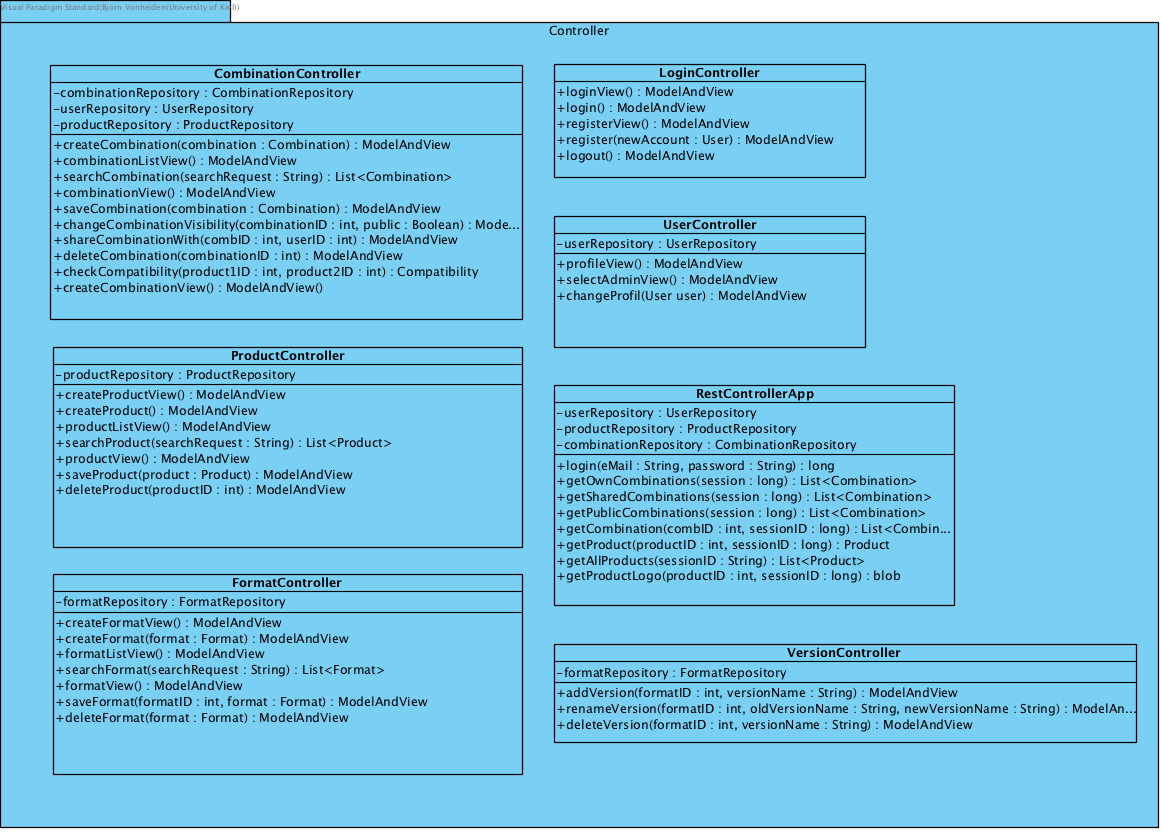
\includegraphics[width=\textwidth]{klassendiagramm/Controller}
	\caption{Klassendiagramm - Controller}
	\label{fig:klassendiagramm-controller}
\end{figure}

\begin{table}[h]
	\centering
	\begin{tabularx}{\textwidth}{X X}
		\rowcolor[HTML]{C0C0C0}
		\textbf{Klassenname} & \textbf{Aufgabe} \\
		Controller.CombinationController & Hier sind alle Controller zur Webapplikation enthalten, welche etwas mit Kombinationen zu tun haben.
		Die Methoden, welche ModelAndView returnen, haben die Annotation '@Controller' und die anderen '@RestController'.
		Die Repositories sind autowired.  \\
		\rowcolor[HTML]{E7E7E7}
		Controller.FormatController  & Diese Klasse enthält alle Controller zur Webapplikation, welche etwas mit Formaten zu tun haben. \\
    	Controller.LoginController & Diese Klasse enthält alle Controller zur Webapplikation, welche etwas mit dem Login zu tun haben.\\
		\rowcolor[HTML]{E7E7E7}
		Controller.ProductController & Diese Klasse enthält analog zur oberen Klasse alle Controller zur Webapplikation, welche etwas mit Diensten zu tun haben. \\
		Controller.RestControllerApp & Diese Klasse enthält alle Controller, welche mit der App kommunizieren.
		Die App schickt dabei GET Anfragen und die URLs fangen mit /App/ an.
		Die Controller sind mit '@RestController' annotiert, es werden also nicht wie bei der Webseite ModelAndViews returnt, sondern in JSON verpackte 		Objekte.
		Die Umwandlung wird von Spring übernommen. \\
		\rowcolor[HTML]{E7E7E7}
		Controller.UserController  & Diese Klasse enthält alle Controller zur Webapplikation, welche etwas mit Benutzern zu tun haben.\\
		Controller.VersionController  & Diese Klasse enthält alle Controller zur Webapplikation, welche etwas mit Versionen von Formaten zu tun haben.\\
		\rowcolor[HTML]{E7E7E7}
	\end{tabularx}
	\caption{Klassenbeschreibung - Controller}
	\label{table:klassenbeschreibung-controller}
\end{table}
\FloatBarrier
\subsection{Repository}
Zusätzlich zu dem 'Model' Package haben wir ein 'Repository' Package, welches zu den Klassen des Models (z.B.: Product) jeweils ein Interface (z.B.: ProductRepository), welches CrudRepository extended.
Die Funktion dieser Interfaces ist die Festlegung der Zugriffsarten auf das Model.
 Da ein Klassendiagramm dazu aber sehr redundant zu dem Model ist und die konkreten Methoden von der Implementierung der Controller abhängig ist, haben wir das hier weggelassen.

\FloatBarrier
\subsection{Security}
In dem 'Security'-Package sollen die Funktionen der Authentification \& Authorization umgesetzt werden. Da viele Funktionen und Klassen schon durch das Spring-Security-Framework gestellt werden und nur konfiguriert bzw. aufgerufen werden müssen und wir uns der Umsetzung noch nicht komplett klar sind, haben wir ein Diagramm an dieser Stelle weggelassen.
So werden wir voraussichtlich beispielsweise für die Http-Requests vorkonfigurieren welche Rollen (siehe Model - User), welche Requests stellen darf.
So unterscheiden wir die Rollen, wie im Pflichtenheft, in unangemeldete Nutzer, eingeloggte Nutzer und Administratoren.
So werden die Seiten: Kombinationen(nur mit den freigegebenen Kombinationen), Dienste, Login und Registrieren, für alle Nutzer freigeben.
Die Seiten: Kombinationen(mit den zusätzlichen Optionen eigene und für einen Freigegebene), Profil und Logout sind für alle angemeldeten Nutzer freigegeben.
Diese erhalten dabei auch Zugriff auf weitere Funktionen wie das Speichern einer Kombination.
Für Administratoren werden zusätzlich noch die Seite Benutzer freigegeben.
Außerdem wird ihm noch der Zugriff auf Administrator-Funktionen wie das Hinzufügen oder Löschen eines Dienstes.
An den meisten Methoden werden wir den Sicherheitsaspekt durch die Security-Annotations des Spring Frameworks umsetzen.


\newpage
\section{App}
\begin{figure}[h]
	\centering
	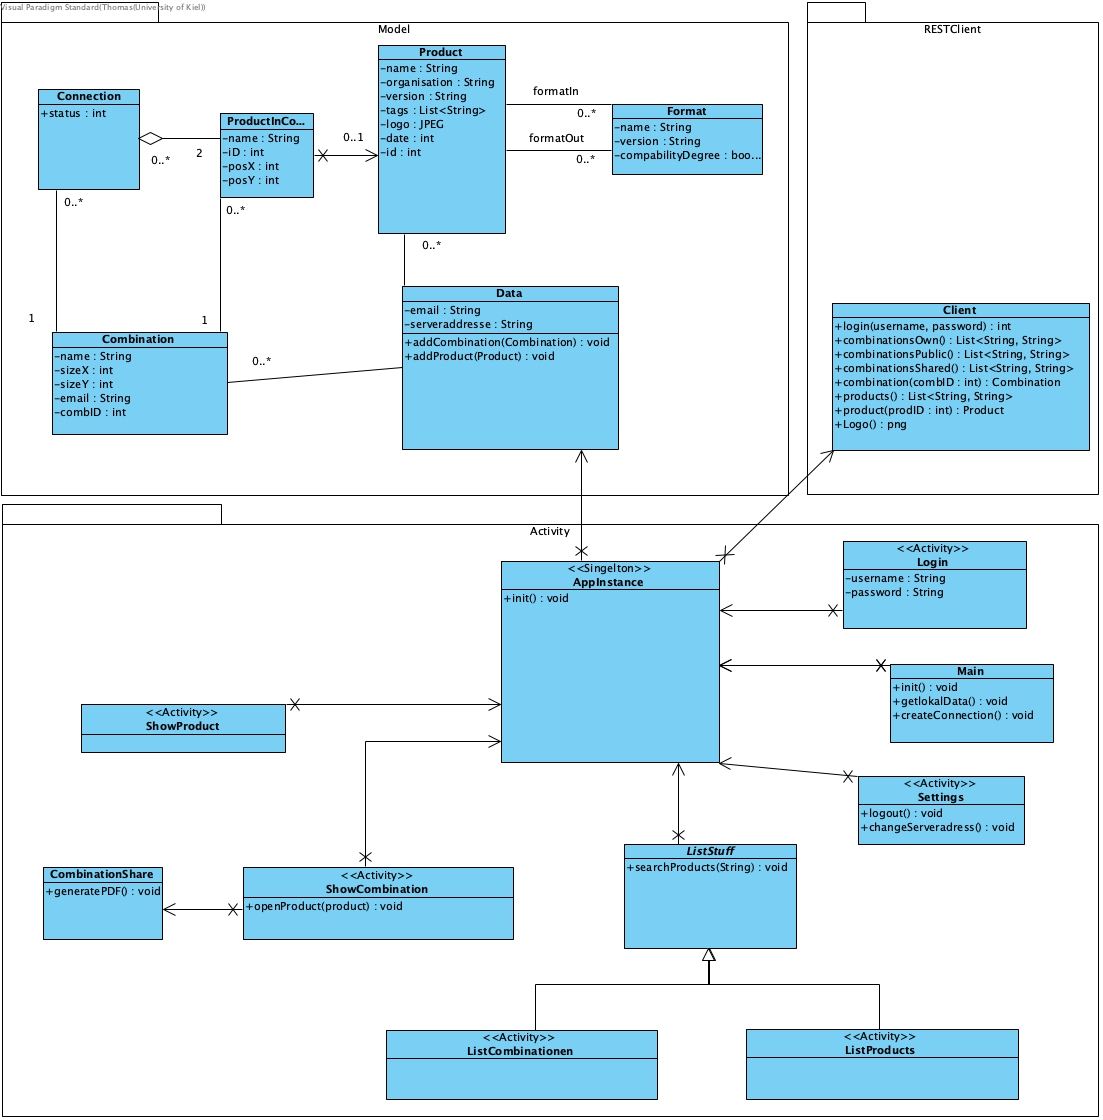
\includegraphics[width=\textwidth]{klassendiagramm/App}
	\caption{Klassendiagramm - App}
	\label{fig:klassendiagramm-app}
\end{figure}

\begin{table}[h]
	\centering
	\begin{tabularx}{\textwidth}{X X}
		\rowcolor[HTML]{C0C0C0}
		\textbf{Klassenname} & \textbf{Aufgabe} \\
		AppInstance & Singelton erlaubt Zugriff auf Data und Client\\
		\rowcolor[HTML]{E7E7E7}
		Client & Übernimmt alle Kommunikationen mit dem Server \\
		CombinationShare & Leitet PDF an das Android System weiter \\
		\rowcolor[HTML]{E7E7E7}
		DataManagement.Combination & Informationen von einer Kombination \\
		DataManagement.Connection  & Informationen von einer Verbindung \\
		\rowcolor[HTML]{E7E7E7}
		DataManagement.Data & Speichert lokal relevante Daten \\
		DataManagement.Format  & Informationen eines Formats\\
		\rowcolor[HTML]{E7E7E7}
		DataManagement.Product & Informationen von einem Dienst \\
		DataManagement.ProductInComb & Speichert ausschließlich die Informationen eines Produkts die zum Visualisieren der Kombination relevant sind.\\
		\rowcolor[HTML]{E7E7E7}
		ListCombination & Darstellung aller möglichen Kombinationen und diese suchbar machen\\
		ListProducts & Darstellung aller möglichen Dienste und diese suchbar machen\\
		\rowcolor[HTML]{E7E7E7}
		ListStuff & Abstrakte Klasse für die Listen(Dienste und Kombinationen)\\
		Login & Stellt den Login bereit \\
		\rowcolor[HTML]{E7E7E7}
		Main & Initialisiert die Applikation \\
		Settings & Stellt Einstellungen für Benutzer bereit \\
    \rowcolor[HTML]{E7E7E7}
		ShowCombination & Generiert Canvas einer Kombination und visualisiert diese  \\
		ShowProduct & Zeigt einen einzelnen Dienst an
	\end{tabularx}
	\caption{Klassenbeschreibung - App}
	\label{table:klassenbeschreibung-app}
\end{table}
